\section{再帰 (Recursion)}
\subsection{再帰への導入}
\begin{frame}[fragile,shrink]
\frametitle{再帰への導入}
  \begin{itemize}
\item 対象(問題)を簡潔に明示的に表す方法
\item たとえば下の絵,ひとつ絵を書いてその中央にその絵を書ている(Droste 効果)
\item 対象を定義するときにより小さい部分を参照して定義する

%\item 関数を合成することで別の関数を定義できる
%\item 複雑な計算を定義する時にはより単純な部分問題に分割して,単純な計算を合成する
  \end{itemize}
  \begin{center}

\includegraphics[scale=0.5]{./Figure/Droste.pdf}
  \end{center}
\end{frame}
\begin{frame}[fragile,shrink]
\frametitle{再帰の例}
  \begin{itemize}
\item 数列 \(a_n=\frac{n(n+1)}{2},\ n\geq 1\)
\item 初項を 1, n 項を \(a_n=n+a_{n-1}\) となる
\item \(n\) 項を決めるのに \(n-1\) 項から決める
\item まだ決まっていない最小の項を既に知っている項から決定する
\item 再帰的定義:
\begin{displaymath}
a(n) = \left\{ \begin{array}{ll}
\displaystyle 1               & \mbox{if }n=1 \\
              n + a(n-1)    & \mbox{otherwise} 
\end{array} \right.
\end{displaymath}
  \end{itemize}
  \begin{columns}
    \begin{column}[t]{0.4\textwidth}
      \begin{center}
\vspace{-2em}
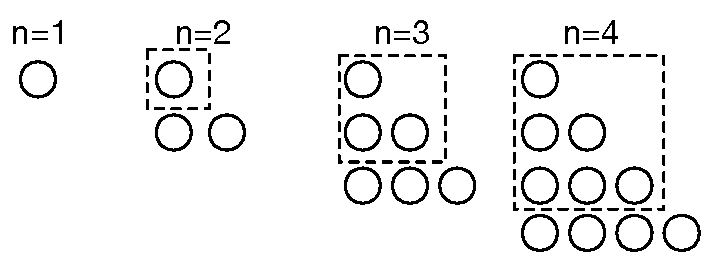
\includegraphics[scale=0.4]{./Figure/elementaryCS-figTriangular.pdf}
      \end{center}
    \end{column}
    \begin{column}[t]{0.4\textwidth}
      \begin{center}
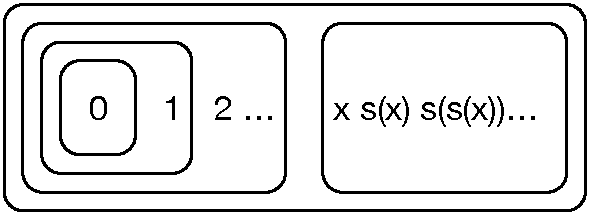
\includegraphics[scale=0.4]{./Figure/elementaryCS-2nd-figRecursion.pdf}
      \end{center}
    \end{column}
  \end{columns}
\end{frame}
\subsection{再帰 (Recursion)}
\begin{frame}[fragile,shrink]
\frametitle{再帰的定義の原理}
  \begin{itemize}
\item 関数 $f$ の定義に $x$ より小さい要素についての評価値を利用して定義することを原始再帰 (primitive recursion) と呼ぶ
\item $f$ が $x$ より小さい値について計算可能であり,いつも同じ値と仮定し, \(f\upharpoonright x\) と書く
\item 定義できた最大の $x$ のつぎの値について定義するというのを繰り返すと全体について定義できる (\(\delta\)-近似)
  \end{itemize}
  \begin{block}{再帰の原理}
\scriptsize
順序数 (自然数は順序数) \(x\) として,
    \begin{center}
\(f(x)=G(f\upharpoonright x)\)
    \end{center}
ここで,\(f\upharpoonright x\) は \(f\) を \(x\) より小さい数に制限したもの, $G$ は計算のしかたを表したもの
  \end{block}
  \begin{center}
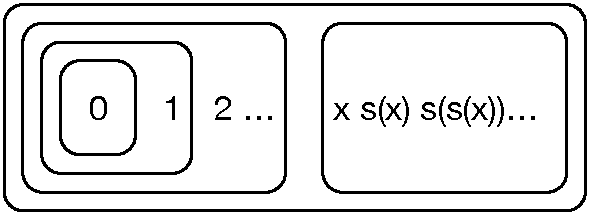
\includegraphics[scale=0.5]{./Figure/elementaryCS-2nd-figRecursion.pdf}
  \end{center}
\end{frame}
\subsection{再帰的定義}
\begin{frame}[fragile,shrink]
\frametitle{関数の再帰的定義}
\framesubtitle{加算,乗算の再帰的定義}
   \begin{itemize}
%\item Basic step と recursive step をそれぞれ定義
\item G に相当するのが \(\operatorname{succ}\)
\item Basic step に近づけるように recursive step を定義
     \begin{itemize}
\item \(a+\operatorname{succ}(b)=\)
     \end{itemize}
  \end{itemize}
\vspace{-1em}
  \begin{center}
  \begin{math}
    \begin{array}{lll}
\mbox{Basic step:}& a+0 & \mbox{if }b=0 \\
\mbox{Recusive step:}& \operatorname{succ}(a+b) & \mbox{otherwise}
    \end{array}
  \end{math}  
  \end{center}
\vspace{-2em}
  \begin{columns}
    \begin{column}[t]{0.4\textwidth}
      \begin{lstlisting}[caption={加算},label=add-rec]
# Recursive definition
import os

def succ (x):
  return(x+1)
def pred (x):
  return(x-1)
def add (a,b):
  if (b==0):
    return(a)
  else:
    return(succ(add(a,pred(b))))
      \end{lstlisting}
    \end{column}
    \begin{column}[t]{0.55\textwidth}
      \begin{lstlisting}[firstnumber=15,caption={乗算},label=mult-rec]
# Multiplication
#
def mult (a,b):
  if (b==0):
    return(0)
  else:
    return(add(add(0,a),mult(a,pred(b))))
      \end{lstlisting}
    \end{column}
  \end{columns}
\end{frame}
\begin{frame}[fragile,shrink]
\frametitle{再帰的定義の例 1}
\framesubtitle{Factorial}
  \begin{itemize}
\item \(n!=n\cdot(n-1)\cdot(n-2)\cdots 3\cdot 2\cdot 1\)
\item \(n!\) を決めるのに \((n-1)!\) の値をつかう
\item G に相当するのが \(n\cdot(n-1)!\) ということ
\item まだ決まっていない最小の値は決まっている値で最大の値のつぎになる
  \end{itemize}
  \begin{columns}[c]
    \begin{column}{0.5\textwidth}
      \begin{lstlisting}[caption={fact.py},label=fact-rec]
def fact (n):
  if (n == 1):
    return(1)
  else:
    return(n*(fact(n-1)))
      \end{lstlisting}
    \end{column}
    \begin{column}{0.45\textwidth}
      \begin{example}[\(4!\)]
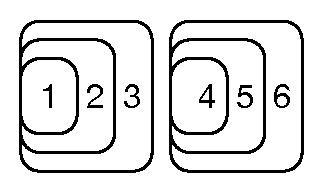
\includegraphics[scale=0.5]{./Figure/elementaryCS-2nd-figFact.eps}
      \end{example}
    \end{column}
  \end{columns}
\end{frame}
\begin{frame}[fragile]
\frametitle{フィボナッチ数}
  \begin{itemize}
\item 突然ですが次の問題を考えてみてください
  \end{itemize}
  \begin{block}{うさぎとフィボナッチ数}
    \begin{itemize}
\item $n$ ヶ月後のうさぎのつがいは何組?
\item 最初一組のつがいだけ
\item 2 ヶ月経つと メス 1 匹を生んでそのつがいが 1 組増える
\item うさぎは決して死なない
    \end{itemize}
  \end{block}
  \begin{center}
    \begin{tabular}{ccccc}
月&生後 0 ヶ月&生後 2 ヶ月以下&合計\\
\hline
1&0&1&1\\
2&0&1&1\\
3&1&1&2\\
4&1&2&3\\
    \end{tabular}
  \end{center}
\end{frame}
\begin{frame}[fragile]
\frametitle{再帰的定義の例 2}
  \begin{itemize}
\item フィボナッチ数\\
    \begin{tabular}{c|c|c|c|c|c}
0&1&2&3&4&5$\cdots$\\
\hline
1&1&2&3&5&8$\cdots$
    \end{tabular}
\item \({\mathop{\mathrm{fib}}}(S(n))\) を決めるのに \({\mathop{\mathrm{fib}}}(n)\) と \({\mathop{\mathrm{fib}}}(n-1)\) を使う
\item G に相当するのが \(n\) と \(n-1\) のフィボナッチ数を足し合わせるということ
  \end{itemize}
  \begin{columns}[c]
    \begin{column}{0.5\textwidth}
      \begin{lstlisting}[caption={フィボナッチ数},label=fib-rec]
def fib (n):
  if (n==0):
    return(0)
  else:
    if (n==1):
      return(1)
    else:
      return(fib(n-1)+fib(n-2))
      \end{lstlisting}
    \end{column}
    \begin{column}{0.45\textwidth}
      \begin{example}[fib\((5)\)]
        \begin{center}
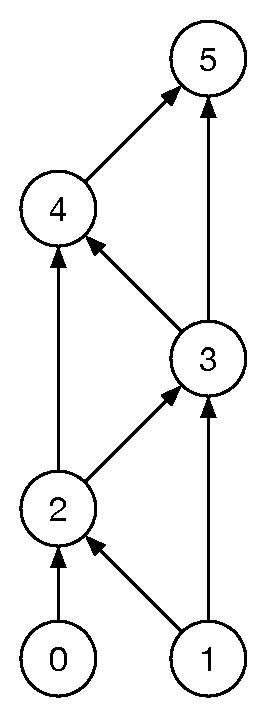
\includegraphics[scale=0.3]{./Figure/elementaryCS-2nd-figFib.eps}
        \end{center}
      \end{example}
    \end{column}
  \end{columns}
\end{frame}
\subsection{木構造}
\begin{frame}[fragile]
\frametitle{Tree (木構造)}
  \begin{itemize}
\item 数以外も
\item Basic step: vertex $r$ は tree
\item Recursive step: \(T_1,T_2,\cdots,T_n\) それぞれ root を \(r_1,r_2,\cdots,r_n\) とする tree として,
\(r\) から \(r_1,r_2,\cdots,r_n\) への edge 追加したものもまた tree である
  \end{itemize}
  \begin{center}
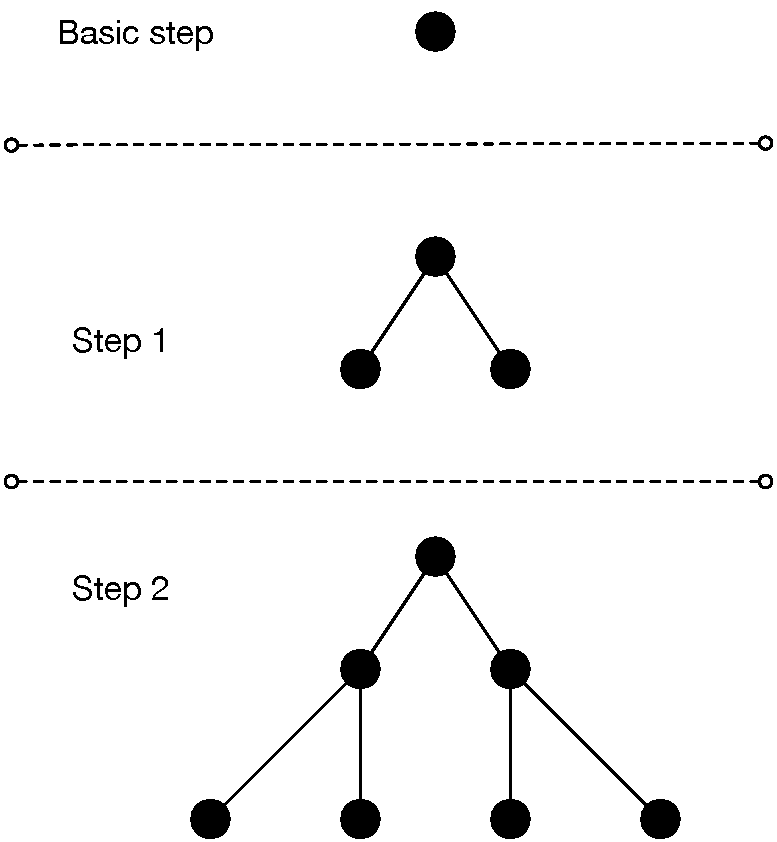
\includegraphics[scale=0.3]{./Figure/elementaryCS-tree.pdf}
  \end{center}
\end{frame}
\begin{frame}[fragile]
\frametitle{集合の再帰的定義}
  \begin{itemize}
\item Basic step: 集合の初期要素を定義
\item Recursive step: 既にわかっている要素から新しい要素を定義する規則
  \end{itemize}
  \begin{example}[文字列の集合\(\Sigma^*\)]
    \begin{itemize}
\item Basic step: \(\epsilon\in\Sigma^*\) (空列 \(\epsilon\) も \(\Sigma^*\) に含まれる)
\item Recursive step: \(a\in\Sigma,w\in\Sigma^*\) ならば \(aw\in\Sigma^*\)
\item E.g.: \(\{\epsilon,\ a,\ aa,\ aaa,\cdots\}\)
    \end{itemize}
  \end{example}
\end{frame}
\begin{frame}[fragile]
\frametitle{再帰は強力な道具}
  \begin{itemize}
\item 最初の元から順番に対象を構成
\item 対象が順番に並べられるなら
\item 問題を解く時も,最も小さい問題の解から順番に全体の解を構成することができる
\item (いつもではないけど)
  \end{itemize}
  \begin{center}
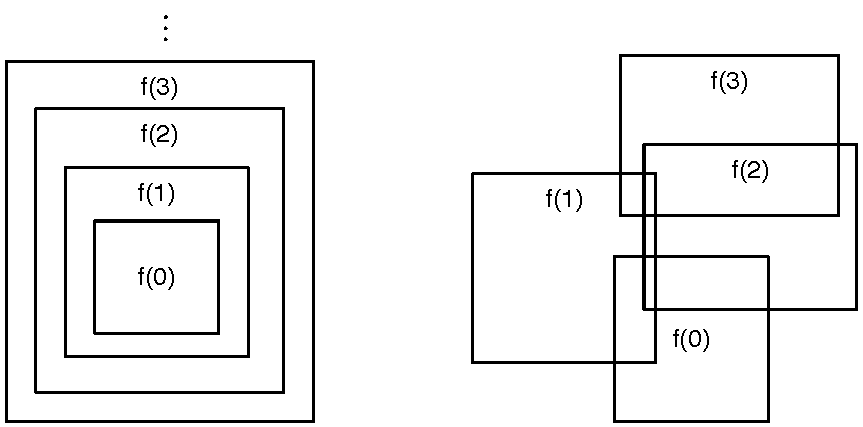
\includegraphics[scale=0.3]{./Figure/Structure.pdf}
  \end{center}
\end{frame}
\begin{frame}[fragile]
\frametitle{宿題 1}
  \begin{itemize}
\item 自然数上の四則演算を再帰で定義せよ(four-ops-rec.py 参照)
\item 先の文字列の集合を参考に文字列の長さを求める関数を再帰的に定義せよ(str\_len.py 参照)
    \begin{itemize}
\item Hint: Basic step を空列は長さ 0 として,recursive step は一文字短い文字列より 1 長い
\item Python では str[1:] とすると文字列の 2 番目以降の文字列を得ることができる
\item 空列は not str で判定
    \end{itemize}
  \end{itemize}
\end{frame}
\section{プログラムとしての再帰}
\subsection{引数の有効範囲 (Scope)}
\begin{frame}[fragile,shrink]
\frametitle{仮引数と実引数}
\scriptsize
  \begin{itemize}
\item CS 第 1 では手続きに名前をつけて抽象化することをみた
\item 関数は 0 個以上の仮引数というものをもつ
    \begin{itemize}
\scriptsize
\item 下の例では {\tt n, eps} などが仮引数
    \end{itemize}
%\item 複数の関数が同じ名前の仮引数を持っていても良い
\item 仮引数は関数の本体で有効である
\item 関数を呼び出したときの値に束縛 (bind) されて,関数の本体では呼び出し時の値に置き換えられる
\item 呼び出し時の値を実引数という
\item 一般に変数は有効範囲 (scope) が決まっている
\item 仮引数は関数本体が有効範囲である
  \end{itemize}
\vspace{-3em}
  \begin{columns}[t]
    \begin{column}{0.5\textwidth}
      \begin{lstlisting}[caption={newton.py},label=newton-rec]
### Newton's method 
def sqrt_iter (guess,n,eps,previous):
  def is_enough (guess,eps,previous):
    return(abs(previous-guess)<(2*eps))
  def improve (guess,n):
    return((guess+(n/guess))/2.0)
  if is_enough(guess,eps,previous):
     return(guess)
  else:
     return(sqrt_iter(improve(guess,n),n,eps,guess))
def sqroot1 (n,eps):
  return(sqrt_iter(1.0,n,(2*eps),0.0))
      \end{lstlisting}
    \end{column}
    \begin{column}{0.45\textwidth}
      \begin{lstlisting}[caption={newton.py},firstnumber=13,label=newton-is_enough-rec]
def sqroot (n):
  ### Machine epsilon
  def eps_m ():
    epsilon, old, prod = 1.0, 0.0, 0.0
    cnt=0
    while (prod!=1.0):
      old = epsilon
      cnt=cnt+1
      epsilon=epsilon/2.0
      prod=epsilon+1.0
    return(old)
  return(sqroot1(n,eps_m()))
      \end{lstlisting}
    \end{column}
  \end{columns}
\end{frame}
\subsection{再帰プログラム}
\begin{frame}[fragile]
\frametitle{プログラムとしての再帰}
  \begin{itemize}
\item プログラムでも関数を定義するときに自身をもちいることができる
\item 下のプログラムを実行してみるので引数の値に注意して見ていてください
\item 関数は定義しただけでは実行されず,呼び出したときはじめて活性化され,仮引数が束縛される
    \begin{itemize}
\item 呼び出し時に環境が作成される: e.g. {\tt n} は 3,2,1 と束縛される
\item その環境のもとで関数の本体が実行される
    \end{itemize}
  \end{itemize}
  \begin{columns}[c]
    \begin{column}{0.6\textwidth}
      \begin{lstlisting}[caption={fact.py},label=fact-with-puts]
# Factorial
def fact (n):
  if (n == 1):
    return(1)
  else:
    return(n*(fact(n-1)))
      \end{lstlisting}
    \end{column}
    \begin{column}{0.35\textwidth}
      \begin{center}
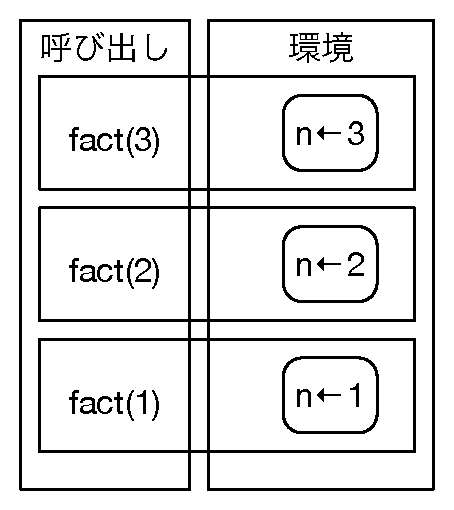
\includegraphics[scale=0.3]{./Figure/elementaryCS-2nd-figStack.eps}
      \end{center}
    \end{column}
  \end{columns}
\end{frame}
\begin{frame}[fragile]
\frametitle{関数の評価と生成プロセス}
  \begin{columns}[c]
    \begin{column}{0.6\textwidth}
      \begin{itembox}{fact(3) の生成プロセス}
        \begin{verbatim}
  fact(3)
=>(3 * fact(2)))
=>(3 * (2 * fact(1))))
=>(3 * (2 * 1)))
=>(3 * 2 ))
=>6
        \end{verbatim}
      \end{itembox}
    \end{column}
    \begin{column}{0.35\textwidth}
      \begin{center}
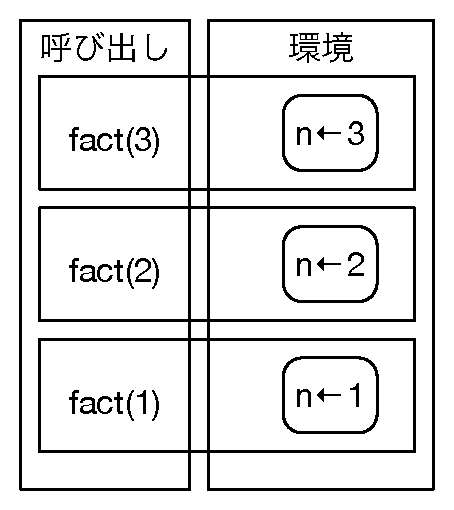
\includegraphics[scale=0.3]{./Figure/elementaryCS-2nd-figStack.eps}
      \end{center}
    \end{column}
  \end{columns}
\end{frame}
%\subsection{分割統治法 (Devide and Conquer)}
%\begin{frame}[fragile]
%\frametitle{分割統治法 (Devide and Conquer)}
%  \begin{itemize}
%\item 分割統治法とは複雑な問題をより簡単な部分問題に分割し,部分問題の解から合成して全体の解を求めるという方法
%\item 分割統治法は再帰プログラムとしてあらわせる
%  \end{itemize}
%  \begin{example}[組合せ (Comination)の部分問題への分割]
%    \begin{itemize}
%\item \(\combination{n}{r}=0\) 
%      \begin{itemize}
%\item \(n,r,n-r<0\) のときの数
%      \end{itemize}
%\item \(\combination{n}{0}=1\) 
%      \begin{itemize}
%\item $n$ 個から $0$ 個取り出したときの数
%      \end{itemize}
%\item \(\combination{n}{r}=\combination{n-1}{r}+\combination{n-1}{r-1}\) 
%      \begin{itemize}
%\item $n$ 個から $1$ 個を除外して残り \(r-1\) を選ぶ場合
%\item $n$ 個から $1$ 個取り出して残り \(r-1\) を選ぶ場合
%      \end{itemize}
%\item \(n,r\) が小さくなっているだけで同じ問題
%    \end{itemize}
%  \end{example}
%\end{frame}
%\begin{frame}[fragile]
%\frametitle{\(\combination{n}{r}\) の定義}
%%  \begin{itemize}
%%\item 以下の定義とプログラムを得る
%%  \end{itemize}
%  \begin{definition}[\(\combination{n}{r}\)]
%\[\combination{n}{r}=\left\{
%      \begin{array}{ll}
%0 & \mbox{if } n,r,n-r<0\\
%1 & \mbox{if } r=0\\
%\combination{n-1}{r-1}+\combination{n-1}{r} & \mbox{otherwise}\\
%      \end{array}
%\right.\]
%  \end{definition}
%  \begin{lstlisting}[caption={組み合わせの数},label=comb]
%# Combination n, r
%def comb (n,r)
%  if ((n-r)<0||n<0||r<0) then
%    return 0
%  else
%    if (r==0) then
%      return 1
%    else
%      return (comb(n-1,r)+comb(n-1,r-1))
%    end
%  end
%end
%### Test Harness
%x = gets().to_i
%y = gets().to_i
%puts "C(n,r)="
%puts(comb(x,y))
%  \end{lstlisting}
%\end{frame}
%\subsection{帰納法 (Induction)}
%\begin{frame}[fragile]
%\frametitle{帰納法の原理}
%  \begin{itemize}
%\item 帰納法は再帰的に定義されたものの性質を証明するテクニック
%\item 再帰的アルゴリズムの正当性を証明するのにも使える
%\item 下に帰納法の原理をあげておきます
%\item \(\operatorname{succ}(y)\) は $y$ のつぎの数という意味です (CS 入門第一の\(+1\) に相当)
%\item 証明したいことがらを \(\phi\) とします
%\item 原理の前提条件を充たすことを示します \(\phi(0)\wedge(\phi(n)\Rightarrow\phi(\operatorname{succ}(n)))\)
%  \end{itemize}
%  \begin{block}{帰納法の原理}
%集合 \(X=\{n\colon \phi(n)\}\) について,もし \(0\in X\) かつ \(\forall y\in X\colon \operatorname{succ}(y)\in X\) であるなら,$X$ はすべての自然数を含む
%  \end{block}
%\end{frame}
\section{Quiz 1}
\begin{frame}[fragile,shrink]
\frametitle{QUIZ 1}
  \begin{itemize}
\item ハノイの塔 (Tower of Hanoi) というパズルを解くプログラムを作成してください
\item 目的:
    \begin{itemize}
\item 柱 1 から柱 2 へ移動
    \end{itemize}
\item 制約:
    \begin{itemize}
\item 柱から柱への移動は一度に 1 枚だけ
\item 大きい円盤をそれより小さい円盤の上にのせてはいけない
    \end{itemize}
\item 4b(CS2) クラスのサイト: \href{https://sites.google.com/presystems.xyz/elementaryCS/}{\beamerbutton{https://sites.google.com/presystems.xyz/elementaryCS}} 
から hanoi-skeleton.py をダウンロードして使ってください
  \end{itemize}
  \begin{center}
\includegraphics[scale=0.4]{./Figure/elementaryCS-2nd-figHanoi.eps}
  \end{center}
\end{frame}
\begin{frame}[fragile,shrink]
\frametitle{Quiz 1 の hint}
  \begin{itemize}
\item Basic step: $1$ 枚の移動
\item Recursive step: $n$ 枚から \(n-1\) 枚の移動
\item hanoi(n,a,b,c) は n 枚のディスクを a から b へ c を使って移動する関数
\item Python でリストに要素を追加するときは append() を使う
  \end{itemize}
  \begin{center}
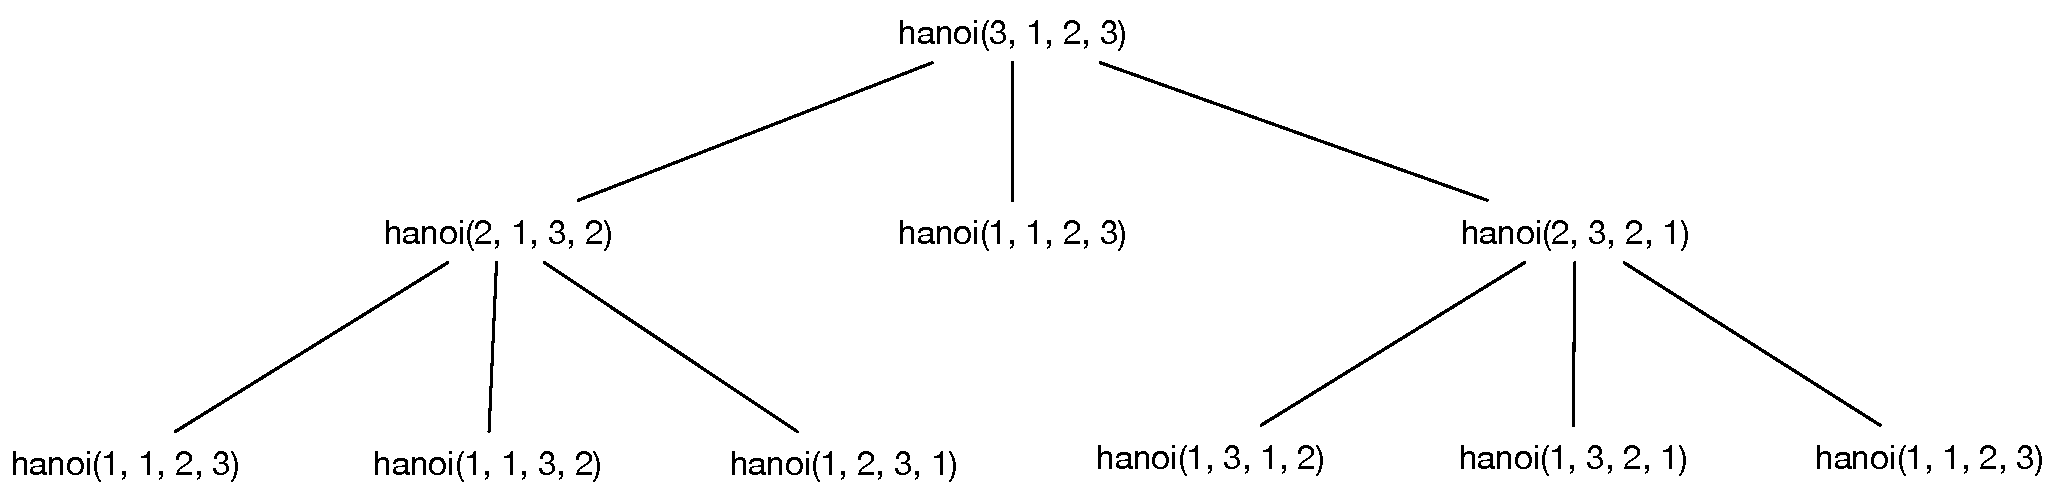
\includegraphics[scale=0.28]{./Figure/elementaryCS-figHanoi-Hint.pdf}
  \end{center}
\end{frame}
\section{繰り返しと再帰}
\subsection{末尾再帰 (Tail Recursion)}
\begin{frame}[fragile,shrink]
\frametitle{繰り返しプログラムと再帰プログラム}
  \begin{itemize}
\item 以前,繰り返しでいろいろな計算を実現しました
\item ここでは繰り返しと再帰の関係について見ていきます
\item \(\operatorname{succ}(y)\) は $y$ のつぎの数という意味で CS 入門第一の\(+1\) に対応
\item \(\operatorname{0}\) は定数 (引数なしの特別な関数)
\item これら初期関数から再帰と関数合成で繰り返しプログラムと同じものが作れます
    \begin{itemize}
\item 関数合成は \(f(g_1(x_1),\ldots,g_n(x_n))\) 
\item 再帰は basic step と recursive step で場合分け
    \end{itemize}
  \end{itemize}
\end{frame}
\begin{frame}[fragile,shrink]
\frametitle{末尾再帰呼び出し (Tail Recursive Call)}
  \begin{itemize}
\item \lstref{fact-rec1}と\lstref{fact-iter}はどちらも再帰的定義ですが計算プロセスに違いがあります
\item \lstref{fact-rec1} は fact(n) を得るために fact(n-1) の後の計算 (n  $\times\,\Box$) を覚えてなければならない
\item \lstref{fact-iter} はその必要はなく,計算の状態``カウンタと途中までの積''を覚えておくだけで良い
\item \lstref{fact-iter} のような形を末尾再帰的といいます
  \end{itemize}
\vspace{-2em}
  \begin{columns}[t]
    \begin{column}{0.45\textwidth}
      \begin{lstlisting}[caption={再帰プロセス版},label=fact-rec1]
# Factorial
def fact (n):
  if (n == 1):
    return(1)
  else:
    return(n*(fact(n-1)))
      \end{lstlisting}
    \end{column}
    \begin{column}{0.5\textwidth}
      \begin{lstlisting}[firstnumber=16,caption={繰り返しプロセス版},label=fact-iter]
# Factorial
def fact_iter (n):
  def fact_iter1 (prod, cnt, max):
    if cnt > max:
      return(prod)
    else:
      return(fact_iter1(prod*cnt,cnt+1,max))
  return(fact_iter1(1,1,n))
      \end{lstlisting}
    \end{column}
  \end{columns}
\end{frame}
\begin{frame}[fragile]
\frametitle{末尾呼び出し (Tail Call)}
  \begin{itemize}
\item 末尾再帰は繰り返し {\tt while, for} に書き換えられます
\item 繰り返しは再帰関数の特別な場合と見なせる
\item 再帰は関数を呼び出すたびに資源を消費するが,繰り返しは一定
  \end{itemize}
  \begin{columns}
    \begin{column}{0.5\textwidth}
      \begin{itembox}{再帰プロセス}
\scriptsize
        \begin{verbatim}
  fact(4)
=>(4 * fact(3))
=>(4 * (3 * fact(2)))
=>(4 * (3 * (2 * fact(1))))
=>(4 * (3 * (2 * 1)))
=>(4 * (3 * 2 ))
=>(4 * 6)
=>24
        \end{verbatim}
      \end{itembox}
    \end{column}
    \begin{column}{0.45\textwidth}
      \begin{itembox}{繰り返しプロセス}
\scriptsize
        \begin{verbatim}
  fact-iter(4)
=>fact-iter1( 1,1,4)
=>fact-iter1( 1,2,4)
=>fact-iter1( 2,3,4)
=>fact-iter1( 6,4,4)
=>fact-iter1(24,5,4)
=>24
        \end{verbatim}
      \end{itembox}
    \end{column}
  \end{columns}
\end{frame}
%
%%% COMPUTER
%
\subsection{コンピュータの中では}
\begin{frame}[shrink]
\frametitle{CPU とメモリ}
  \begin{itemize}
\item コンピュータの命令自体も符号化されてます
\item CPU (Central Processing Unit) ごとに命令セットも符号も異なっています
\item ここでは CPU が命令を実行するサイクルについて見てみます
  \end{itemize}
  \begin{center}
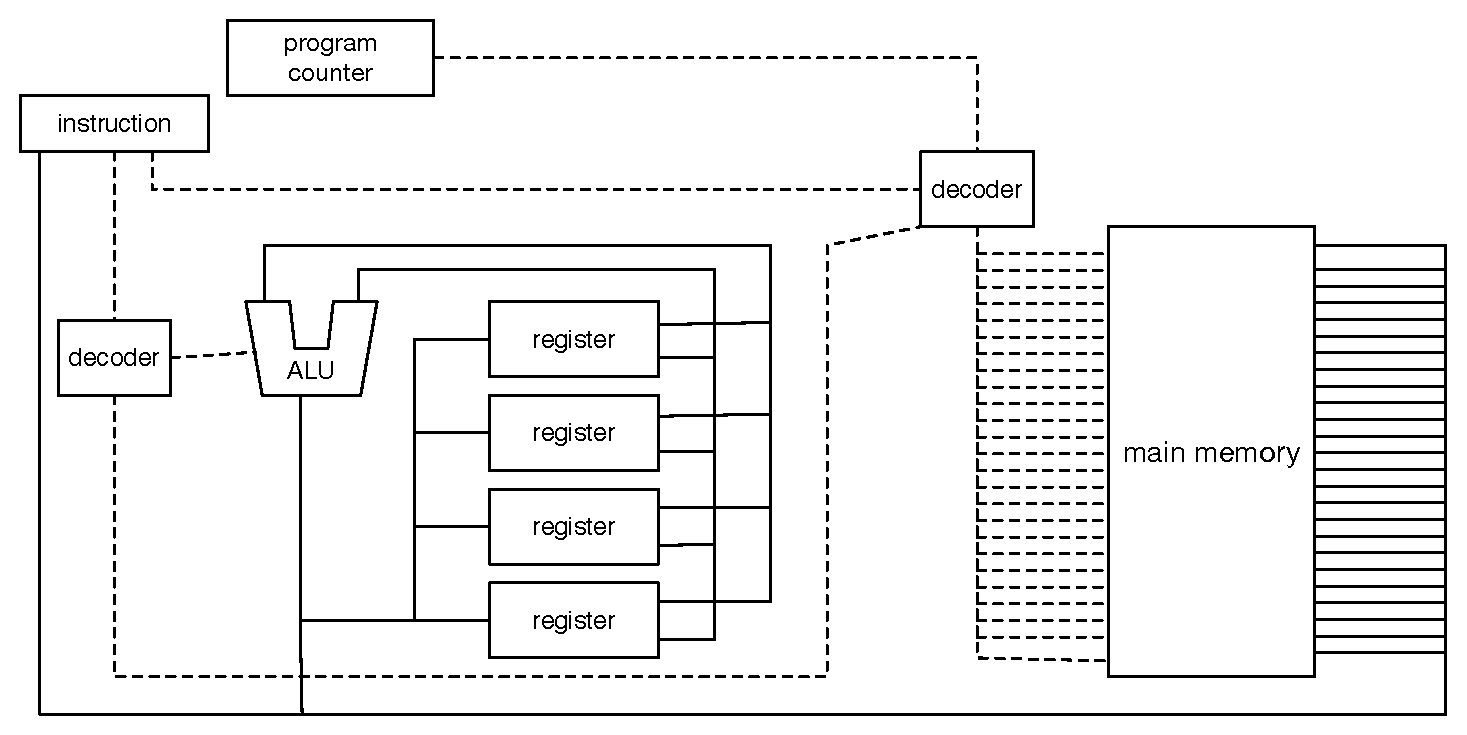
\includegraphics[scale=0.3]{./Figure/elementaryCS-figCPU}
  \end{center}
\end{frame}
\begin{frame}[shrink]
\frametitle{演算のサイクル}
  \begin{enumerate}
\scriptsize
\item Instruction に命令をフェッチ
\item メインメモリからレジスタにデータを移動
\item ALU (Arithmetic and Logic Unit) がレジスタからデータを取り出す
\item ALU で演算
\item 結果をレジスタに書き込む
\item レジスタからメインメモリにデータを移動
\item ADD cx dx bx という命令を例にすると下図のようになります
  \end{enumerate}
  \begin{center}
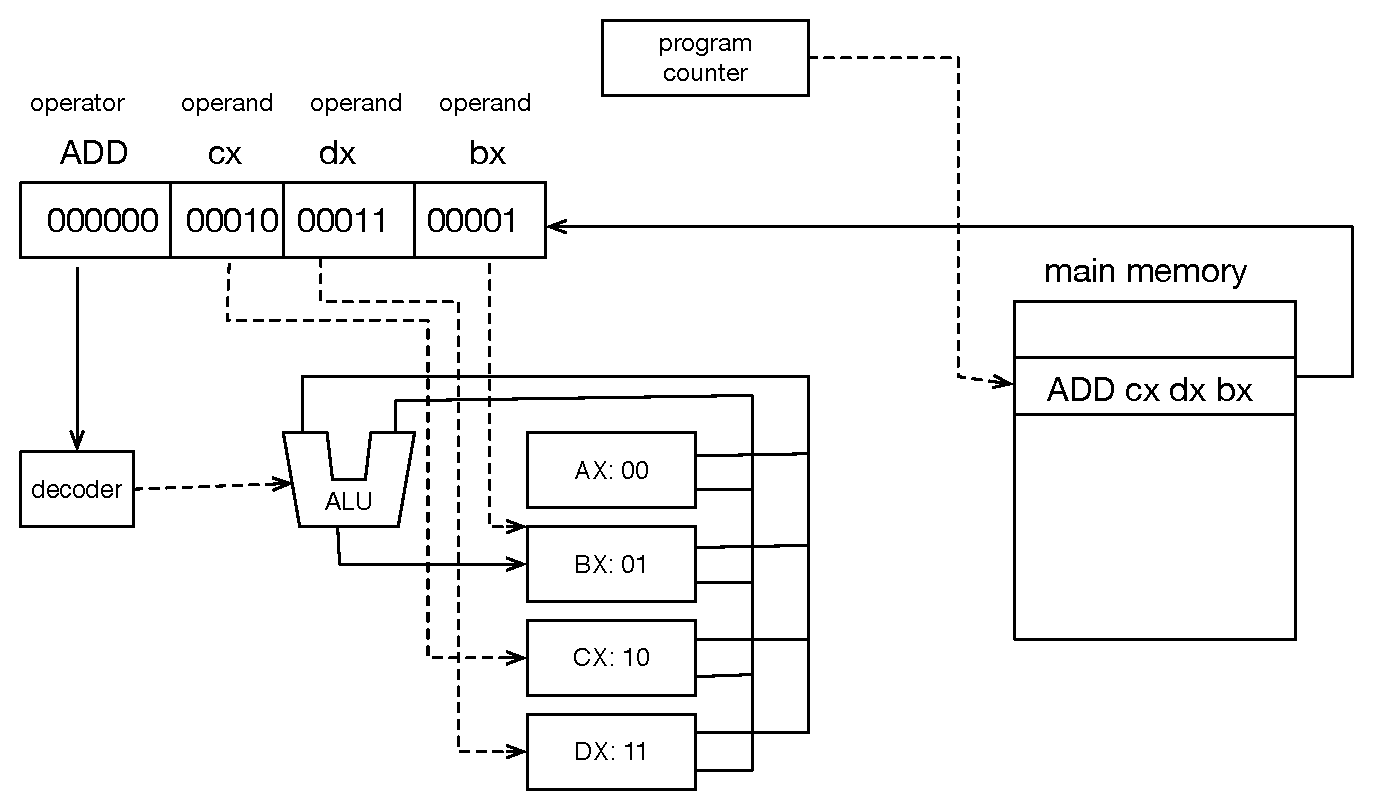
\includegraphics[scale=0.3]{./Figure/elementaryCS-figCycle}
  \end{center}
\end{frame}
\begin{frame}[shrink]
\frametitle{関数を呼び出したとき}
  \begin{itemize}
\item 関数を呼び出すたびに下図の右側のように実行時スタックの領域に保存する
    \begin{itemize}
\item 活性レコード (activation record) という
    \end{itemize}
\item 終了すれば活性レコードは開放される
\item 多くのプログラミング言語は末尾再帰を繰り返しに変換してくれないので繰り返し構文が用意されている
  \end{itemize}
  \begin{center}
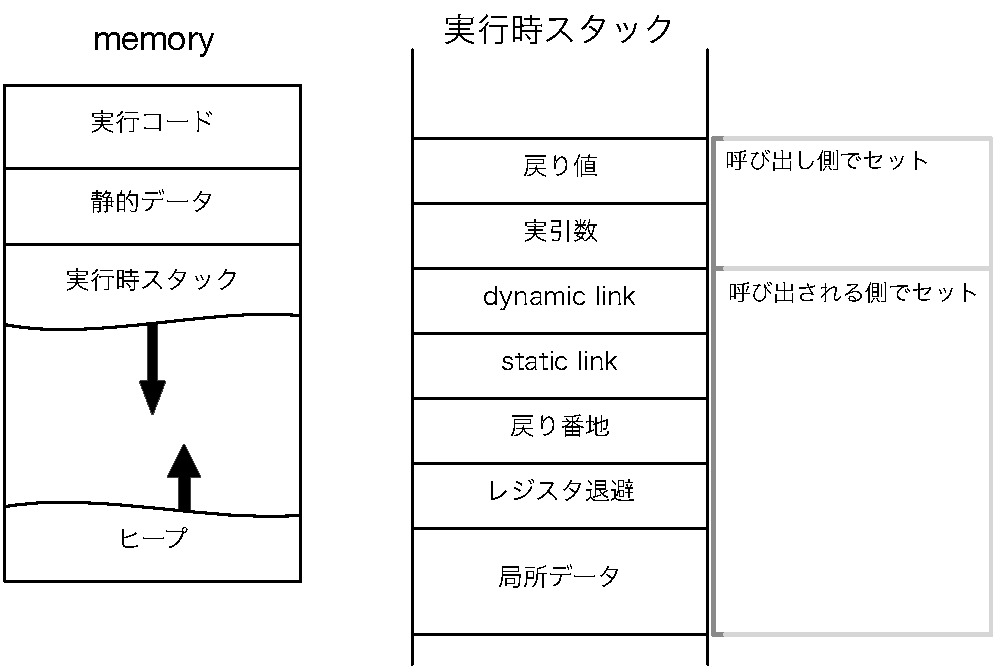
\includegraphics[scale=0.3]{./Figure/elementaryCS-figMemory}
  \end{center}
\end{frame}
\section{再帰のまとめ}
\begin{frame}[fragile]
\frametitle{再帰のまとめ}
  \begin{itemize}
\item 再帰とはある問題をそれより簡単な同じ問題に分解して問題を解く方法
\item 既にわかっているそれより前のものから求める
\item 一見複雑な問題も再帰的に定義すると単純な計算で解ける
\item それ以上分割出来ない問題を解き,結果からより大きい問題の結果を得るというもの (分割統治法 (Divide and Conquer) と呼ばれる)
\item E.g. Quiz 1 では複雑な問題をより小さい同じ問題に分解して解いていっている
\item 再帰は非常に強力な解法になる
  \end{itemize}
\end{frame}
